\newif\ifglobal

%%%%%%%%%%%%%%%%%%%%%%%
%%% Compile to view %%%
%%%%%%%%%%%%%%%%%%%%%%%

%%%%%%%%%%%%%%%%%%%%%%%%%%%%%%%%%%%%%%%%%%%%%%%%%%%
%%% Readme:                                     %%%
%%% https://www.overleaf.com/read/bwdjvfjksvjy/ %%%
%%%%%%%%%%%%%%%%%%%%%%%%%%%%%%%%%%%%%%%%%%%%%%%%%%%

% >>> M?: marks a module setting number or important notice

% >>> M4: Set {./relative-path} to external files for this module <<<
\def \modulefiles {./03-I2S}
% To add an external file, use:
% (Replace '---' with actual filename)
% '\input{\modulefiles/tables/---.tex}' for tables
% '\includegraphics{\modulefiles/figures/---}' for figures
% '\subfile{\modulefiles/---}' for register files

% >>> M1: This module is in global project? <<<
% 'YES' - uncomment; 'NO' - comment out
\globaltrue

\ifglobal
    \documentclass[main\_\_CN.tex]{subfiles}

\else
    % Font "FandolSong-Regular" used by ctex does not have GSUB table.
    % It causes warnings that do not affect compilation and can be ignored.
    \PassOptionsToPackage{quiet}{fontspec}

    \documentclass[openany, 10pt]{book}

    % >>> M2: In ./00-shared/preamble-trm-module, also find
    %         settings for visibility of todo notes, watermark <<<
    \usepackage{preamble-trm-module}


    % Enable Chinese typesetting
    \usepackage{ctex}

    % >>> M3: Temporary labels in Chinese
    %         you can add your own labels there <<<
    \myexternaldocument{./00-shared/temp-labels-en}

\fi %\ifglobal


\setcounter{secnumdepth}{4}

% >>> M4: Set {./relative-path} to external files for this module <<<
% \def \modulefiles {./03-I2S}
% To add an external file, use:
% (Replace '---' with actual filename)
% '\input{\modulefiles/tables/---.tex}' for tables
% '\includegraphics{\modulefiles/figures/---}' for figures
% '\subfile{\modulefiles/---}' for register files


% >>> M5: If this module needs any updates in
% './00-shared/preamble-trm-module.sty'
% (include additional package, etc.), contact your module PM
% or create the file './00-shared/changelog.tex' make the
% necessary updates yourself and document them in this file <<<


\begin{document}


% Sets language into which pre-defined bits of text are translated
\selectlanguage{english}

% Do not delete this block
\ifglobal
% Add the following front matter if
% this module is outside of global project
\else
    \InputIfFileExists{readme}{}{}
    {\let\clearpage\relax \listoftodos}
    \tableofcontents
    %\listoftables
    %\listoffigures
\fi


%%%%%%%%%%%%%%%%%%%%%%%%%
%%% TRM Module Begins %%%
%%%%%%%%%%%%%%%%%%%%%%%%%


\hypertarget{i2s}{}
\chapter{I2S Controller (I2S)}
\label{mod:i2s}

\section{Overview}
\chipname{} has two built-in I2S interfaces (i.e. I2S\regindex{0} and I2S\regindex{1}), which provides a flexible communication interface for streaming digital data in multimedia applications, especially digital audio applications.

The I2S standard bus defines three signals: a bit clock signal (BCK), a channel/word select signal (WS), and a serial data signal (SD). A basic I2S data bus has one master and one slave. The roles remain unchanged throughout the communication. The I2S module on \chipname{} provides separate transmit (TX) and receive (RX) units for high performance.

\begin{tiplisting}
The information provided in this chapter applies to I2S\regindex{0} and I2S\regindex{1}. Unless otherwise indicated, I2S\regindex{n} or I2S in this chapter refer to both I2S\regindex{0} and I2S\regindex{1}.
\end{tiplisting}

\section{Terminology}

To better illustrate the functionality of I2S\regindex{n}, the following terms are used in this chapter.

\begin{longtable}[c]{ R{4cm} p{10cm} }

\textbf{Master mode}     & As a master, I2S\regindex{n} outputs BCK/WS signals, and sends data to or receives data from a slave. \\
\textbf{Slave mode}      & As a slave, I2S\regindex{n} inputs BCK/WS signals, and receives data from or sends data to a master. \\
\textbf{Full-duplex} & The sending line and receiving line between the master and the
slave are independent. Sending data and receiving data happen
at the same time.\\
\textbf{Half-duplex} & Only one side, the master or the slave, sends data first, and the
other side receives data. Sending data and receiving data can not
happen at the same time.\\
\textbf{TDM RX mode} & In this mode, pulse code modulated (PCM) data is received and stored into memory via DMA, in a way of time division multiplexing (TDM). The signal lines include: BCK, WS, and DATA. Data from 16 channels at most can be received. TDM Philips standard, TDM MSB alignment standard, TDM PCM standard are supported in this mode, depending on user configuration.\\
\textbf{PDM RX mode} & In this mode, pulse density modulation (PDM) data is received and stored into memory via DMA. The signal lines include: WS and DATA. PDM standard is supported in this mode by user configuration.\\
\textbf{TDM TX mode} & In this mode, pulse code modulated (PCM) data is sent from memory via DMA, in a way of time division multiplexing (TDM). The signal lines include: BCK, WS, and DATA. Data up to 16 channels can be sent. TDM Philips standard, TDM MSB alignment standard, TDM PCM standard are supported in this mode, depending on user configuration.\\
\textbf{PDM TX mode} & In this mode, pulse density modulation (PDM) data is sent from memory via DMA. The signal lines include: WS and DATA. PDM standard is supported in this mode by user configuration.\\
\textbf{PCM-to-PDM TX mode (for I2S\regindex{0} only)} & In this mode, I2S\regindex{0} as a \textbf{master}, converts the pulse code modulated (PCM) data from memory via DMA into pulse density modulation (PDM) data, and then sends the data out. The signal lines include: WS and DATA. PDM standard is supported in this mode by user configuration.\\
\textbf{PDM-to-PCM RX mode (for I2S\regindex{0} only)} & In this mode, I2S\regindex{0} works as a master or a \textbf{slave}. Pulse density modulation (PDM) data is received, converted into pulse code modulated (PCM) data, and then stored into memory via DMA. The signal lines include: WS and DATA. PDM standard is supported in this mode by user configuration.\\
\end{longtable}


\section{Features}

I2S\regindex{n} has the following features:

\begin{itemize}
    \item Master mode and slave mode
    \item Full-duplex and half-duplex communications
    \item Separate TX unit and RX unit, independent of each other
    \item TX unit and RX unit to work independently and simultaneously
    \item A variety of audio standards supported:
    \begin{itemize}
        \item TDM Philips standard
        \item TDM MSB alignment standard
        \item TDM PCM standard
        \item PDM standard
    \end{itemize}
    \item Various TX/RX modes supported:
        \begin{itemize}
        \item TDM TX mode
        \item TDM RX mode
        \item PDM TX mode
        \item PDM RX mode
        \item PCM-to-PDM TX mode (for I2S\regindex{0} only)
        \item PDM-to-PCM RX mode (for I2S\regindex{0} only)
    \end{itemize}
    \item Configurable high-precision sample clock
    \item Various frequencies supported: 8 kHz, 16 kHz, 32 kHz, 44.1 kHz, 48 kHz, 88.2 kHz, 96 kHz, 128 kHz, and 192 kHz (192 kHz is not supported in 32-bit slave mode).
    \item 8-/16-/24-/32-bit data communication
    \item DMA access
    \item Standard I2S interface interrupts
\end{itemize}
\section{System Architecture}
\begin{figure}[H]
    \centering
    \fbox{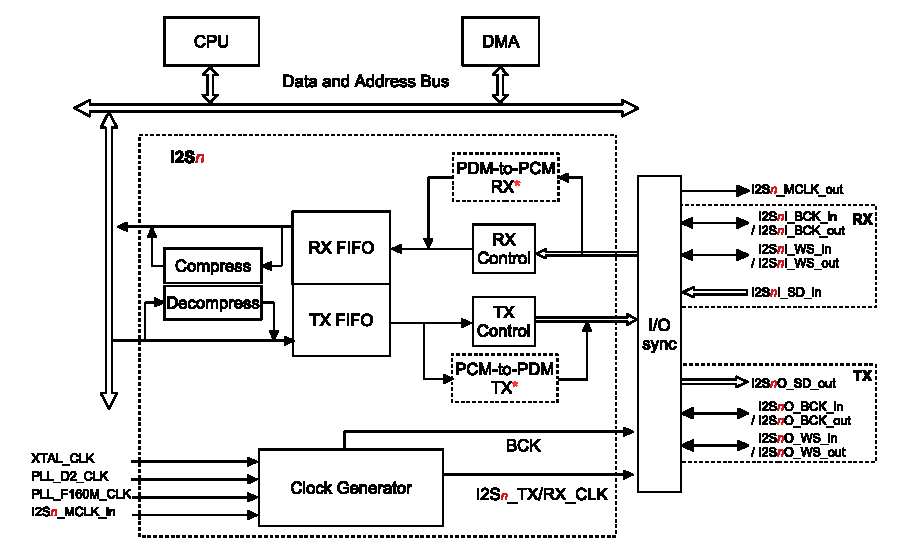
\includegraphics[width=0.9\textwidth]{03-I2S/figures/i2s_arch_20220729.eps}}\\
    Note: PDM-to-PCM RX and PCM-to-PDM TX are only supported by I2S\regindex{0}.
    \caption{\chipname{} I2S System Diagram}
    \label{Figure:i2s_arch}
\end{figure}

Figure  \ref{Figure:i2s_arch} shows the structure of  \chipname{} I2S\regindex{n} module, consisting of:
\begin{itemize}
    \item TX unit (TX control)
    \item RX unit (RX control)
    \item Input and Output Timing unit (I/O sync)
    \item Clock Divider (Clock Generator)
    \item 64 x 32-bit TX FIFO
    \item 64 x 32-bit RX FIFO
    \item Compress/Decompress units
\end{itemize}
\chipname{} I2S\regindex{n} module supports direct access (GDMA) to internal memory and external memory, see Chapter  \ref{mod:dma} \textit{\nameref{mod:dma}}.


Both the TX unit and the RX unit have a three-line interface that includes a bit clock line (BCK), a word select line (WS), and a serial data line (SD). The SD line of the TX unit is fixed as output, and the SD line of the RX unit as input. BCK and WS signal lines for TX unit and RX unit can be configured as master output mode or slave input mode.



The signal bus of I2S\regindex{n} module is shown at the right part of Figure  \ref{Figure:i2s_arch}. The naming of these signals in RX and TX units follows the pattern: I2S\regindex{n}\textcolor{red}{A}\_\textcolor{red}{B}\_\textcolor{red}{C}, for example, I2S\regindex{n}\textcolor{red}{I}\_\textcolor{red}{BCK}\_\textcolor{red}{in}.

\begin{itemize}
    \item ``A": direction of data bus
    \begin{itemize}
        \item ``I": input, receiving
        \item ``O": output, transmitting
    \end{itemize}
    \item ``B": signal function
    \begin{itemize}
        \item bit clock signal (BCK)
        \item word select signal (WS)
        \item serial data signal (SD)
    \end{itemize}
    \item ``C": signal direction
    \begin{itemize}
        \item ``in": input signal into I2S\regindex{n} module
        \item ``out": output signal from I2S\regindex{n} module
    \end{itemize}
\end{itemize}

Table \ref{table:I2S 信号总线描述} provides a detailed description of I2S\regindex{n} signals.


\begin{table}[H]
    \centering
    \caption{I2S\regindex{n} Signal Description}
    \label{table:I2S 信号总线描述}
    \begin{threeparttable}
    \begin{tabular}{|p{2.6cm}|p{1.5cm}|p{11cm}| }
    \hline
    \rowcolor{lightgray}
    \textbf{Signal\tnote{*}}&\textbf{Direction}&\textbf{Function}\\
    \hline
    I2S\regindex{n}I\_BCK\_in & Input & In slave mode, inputs BCK signal for RX unit.\\
    \hline
    I2S\regindex{n}I\_BCK\_out& Output & In master mode, outputs BCK signal for RX unit.\\
    \hline
    I2S\regindex{n}I\_WS\_in & Input & In slave mode, inputs WS signal for RX unit.\\
    \hline
    I2S\regindex{n}I\_WS\_out& Output & In master mode, outputs WS signal for RX unit.\\\hline
    I2S\regindex{n}I\_Data\_in& Input & Works as the serial input data bus for RX unit.\\\hline
    I2S\regindex{n}O\_Data\_out& Output & Works as the serial output data bus for TX unit.\\\hline
    I2S\regindex{n}O\_BCK\_in& Input & In slave mode, inputs BCK signal for TX unit. \\\hline
    I2S\regindex{n}O\_BCK\_out& Output & In master mode, outputs BCK signal for TX unit. \\\hline
    I2S\regindex{n}O\_WS\_in& Input & In slave mode, inputs WS signal for TX unit.\\\hline
    I2S\regindex{n}O\_WS\_out& Output & In master mode, outputs WS signal for TX unit.\\\hline
    I2S\regindex{n}\_MCLK\_in& Input & In slave mode, works as a clock source from the external master.\\\hline
    I2S\regindex{n}\_MCLK\_out& Output & In master mode, works as a clock source for the external slave.\\\hline
    I2S\regindex{0}I\_Data1\_in& Input & In PDM-to-PCM RX mode, works as the serial input data line for RX unit. \\\hline
    I2S\regindex{0}I\_Data2\_in& Input & In PDM-to-PCM RX mode, works as the serial input data line for RX unit.\\\hline
    I2S\regindex{0}I\_Data3\_in& Input & In PDM-to-PCM RX mode, works as the serial input data line for RX unit.\\\hline
    I2S\regindex{0}O\_Data1\_out& Output & In PCM-to-PDM TX mode, works as the serial output data line for TX unit. \\\hline
    \end{tabular}
    \begin{tablenotes}
    \item[*] Any required signals of I2S\regindex{n} must be mapped to the chip's pins via GPIO matrix, see Chapter \ref{mod:iomuxgpio} \textit{\nameref{mod:iomuxgpio}}.
    \end{tablenotes}

        \end{threeparttable}
\end{table}


\section{Supported Audio Standards} \label{I2S_supported_protocal}

\chipname{} I2S\regindex{n} supports multiple audio standards, including TDM Philips standard, TDM MSB alignment standard, TDM PCM standard, and PDM standard.

Select the standard by configuring the following bits:
\begin{itemize}
    \item \hyperref[fielddesc:I2SRXMSBSHIFT]{I2S\_TX/RX\_TDM\_EN}
    \begin{itemize}
        \item 0: disable TDM mode.
        \item 1: enable TDM mode.
    \end{itemize}
    \item \hyperref[fielddesc:I2SRXMSBSHIFT]{I2S\_TX/RX\_PDM\_EN}
    \begin{itemize}
        \item 0: disable PDM mode.
        \item 1: enable PDM mode.
    \end{itemize}
    \item \hyperref[fielddesc:I2SRXMSBSHIFT]{I2S\_TX/RX\_MSB\_SHIFT}
    \begin{itemize}
        \item 0: WS and SD signals change simultaneously, i.e. enable MSB alignment standard.
        \item 1: WS signal changes one BCK clock cycle earlier than SD signal, i.e. enable Philips standard or select PCM standard.
    \end{itemize}
    \item \hyperref[fielddesc:I2SRXPCMBYPASS]{I2S\_TX/RX\_PCM\_BYPASS}
    \begin{itemize}
        \item 0: enable PCM standard.
        \item 1: disable PCM standard.
    \end{itemize}
\end{itemize}

\subsection{TDM Philips Standard}

Philips specifications require that WS signal changes one BCK clock cycle earlier than SD signal on BCK falling edge, which means that WS signal is valid from one clock cycle before transmitting the first bit of channel data and changes one clock before the end of channel data transfer. SD signal line transmits the most significant bit of audio data first.

Compared with Philips standard, TDM Philips standard supports multiple channels, see Figure  \ref{Figure:i2s_phillips_standard}.
\begin{figure}[H]
    \centering
    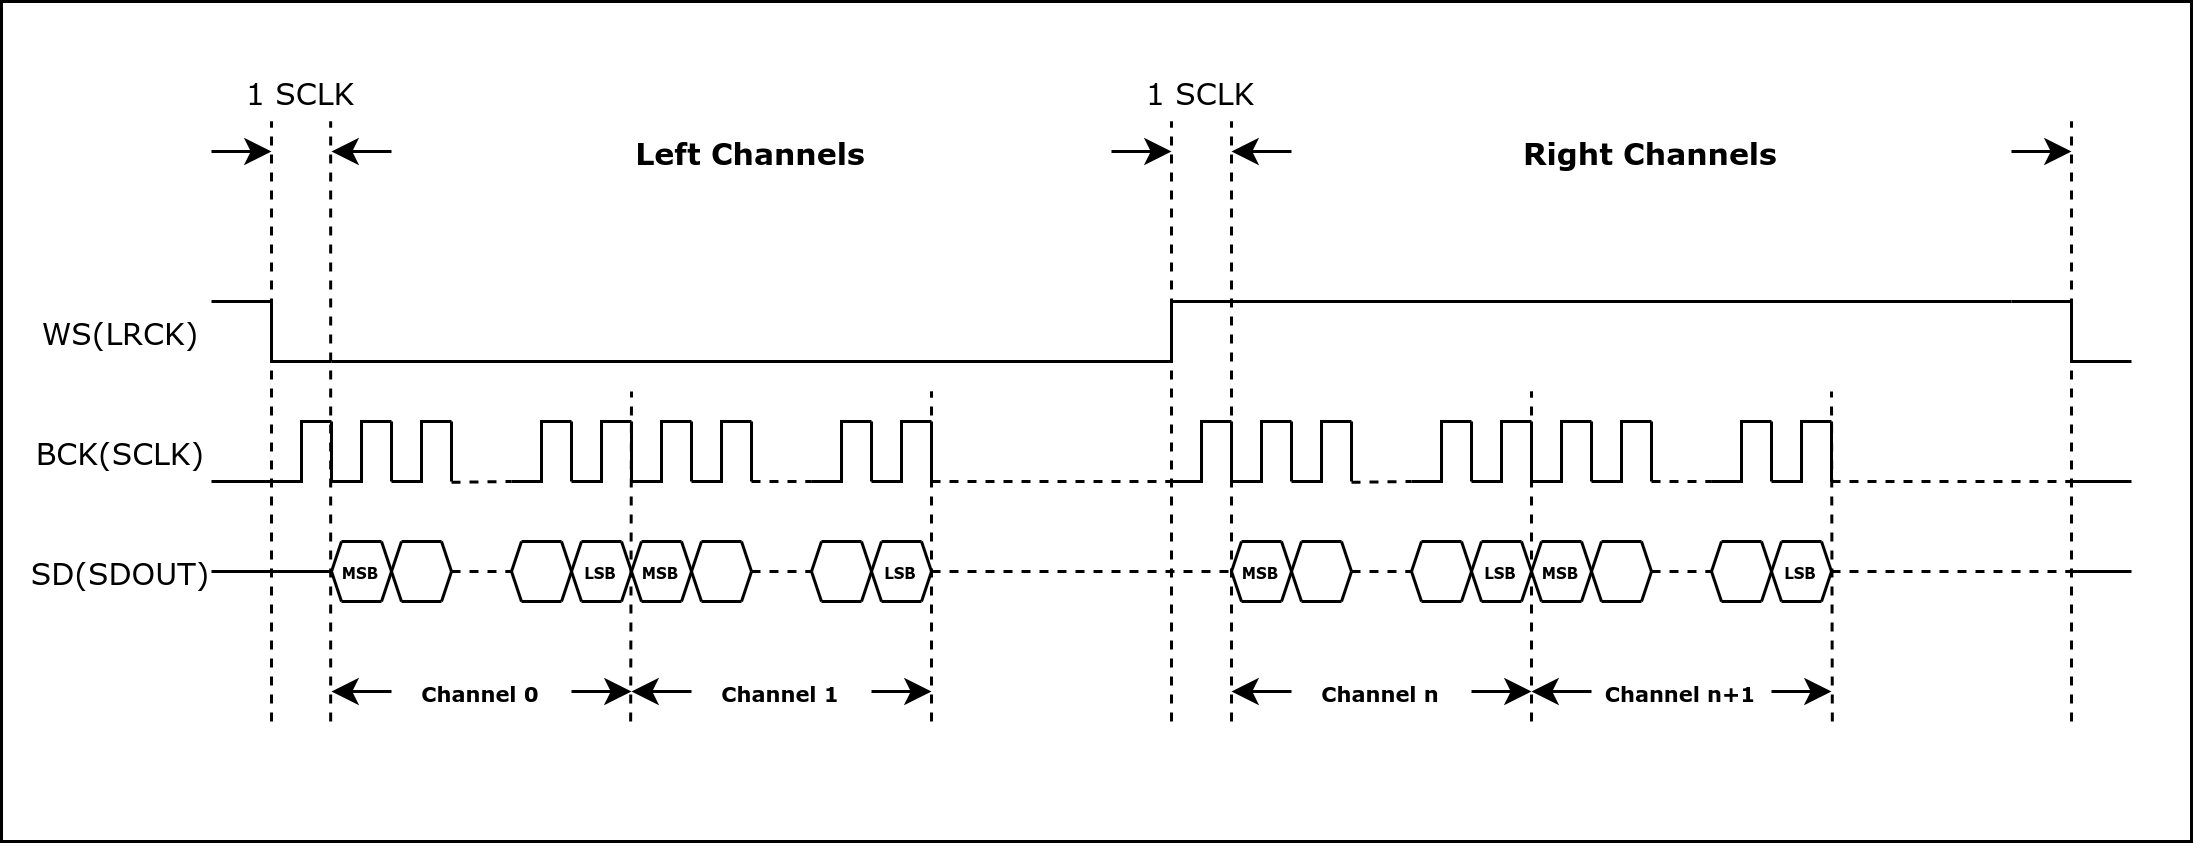
\includegraphics[width=1.0\textwidth]{03-I2S/figures/i2s_tdm_phillips_mode.png}
    \caption{TDM Philips Standard Timing Diagram}
    \label{Figure:i2s_phillips_standard}
\end{figure}

\subsection{TDM MSB Alignment Standard}

MSB alignment specifications require WS and SD signals change simultaneously on the falling edge of BCK. The WS signal is valid until the end of channel data transfer. The SD signal line transmits the most significant bit of audio data first.

Compared with MSB alignment standard, TDM MSB alignment standard supports multiple channels, see Figure  \ref{Figure:i2s_MSB_32_mode}.

\begin{figure}[H]
    \centering
    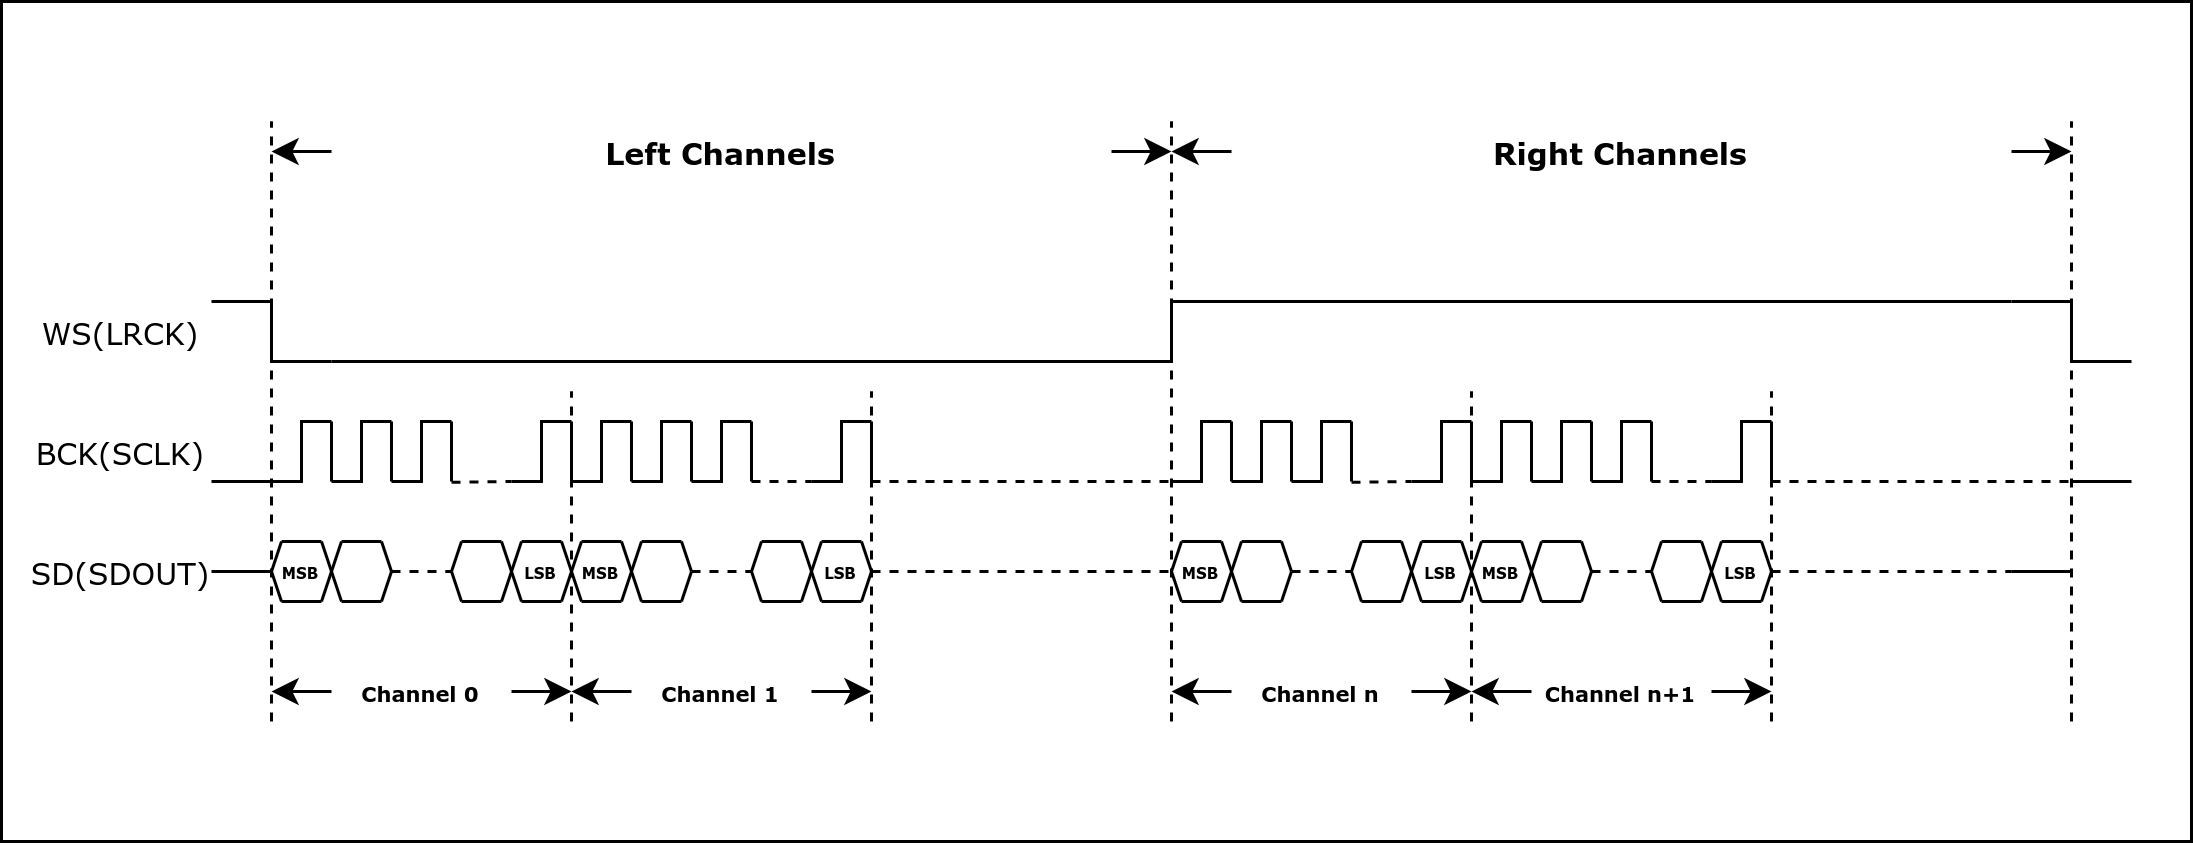
\includegraphics[width=1.0\textwidth]{03-I2S/figures/i2s_tdm_msb_mode.png}
    \caption{TDM MSB Alignment Standard Timing Diagram}
    \label{Figure:i2s_MSB_32_mode}
\end{figure}

\subsection{TDM PCM Standard}

Short frame synchronization under PCM standard requires WS signal changes one BCK clock cycle earlier than SD signal on the falling edge of BCK, which means that the WS signal becomes valid one clock cycle before transferring the first bit of channel data and remains unchanged in this BCK clock cycle. SD signal line transmits the most significant bit of audio data first.

Compared with PCM standard, TDM PCM standard supports multiple channels, see Figure  \ref{Figure:i2s_pcm_mode}.

\begin{figure}[H]
    \centering
    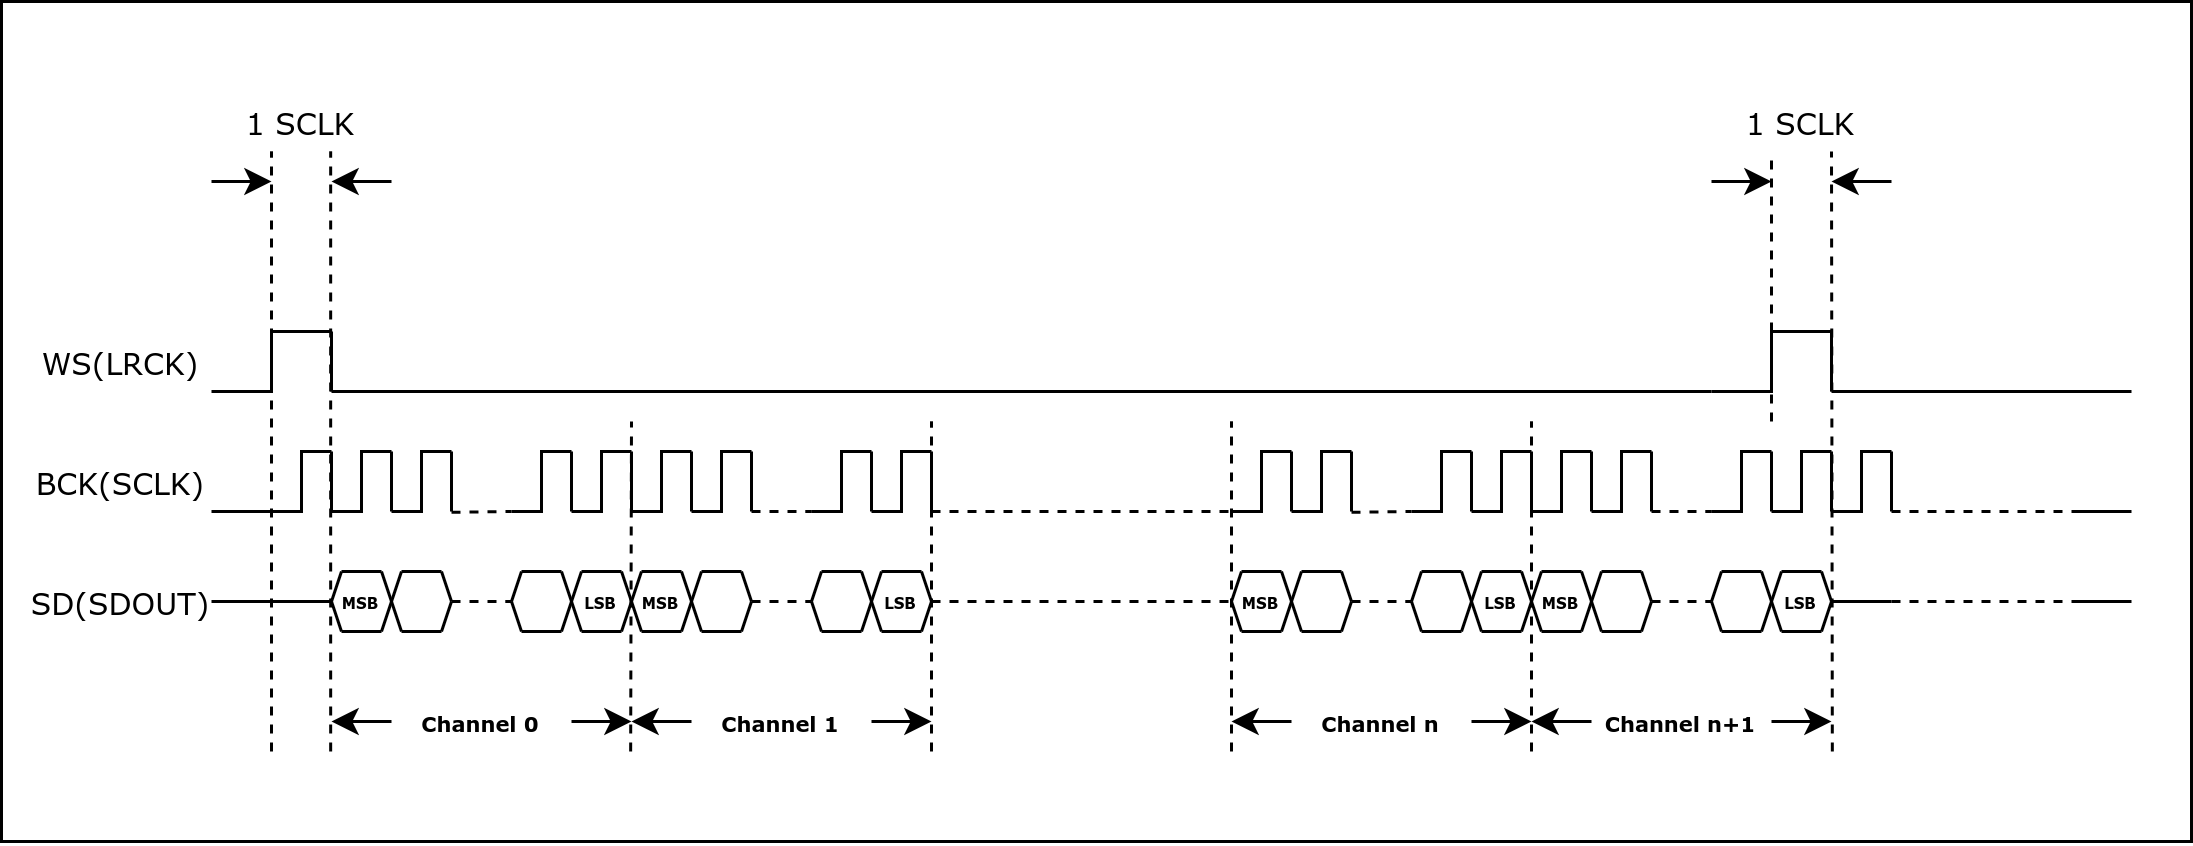
\includegraphics[width=1.0\textwidth]{03-I2S/figures/i2s_tdm_pcm_mode.png}
    \caption{TDM PCM Standard Timing Diagram}
    \label{Figure:i2s_pcm_mode}
\end{figure}

\subsection{PDM Standard}
Under PDM standard, WS signal changes continuously during data transmission. The low-level and high-level of this signal indicates the left channel and right channel, respectively. WS and SD signals change simultaneously on the falling edge of BCK, see Figure  \ref{Figure:i2s_pdm_mode}.

\begin{figure}[H]
    \centering
    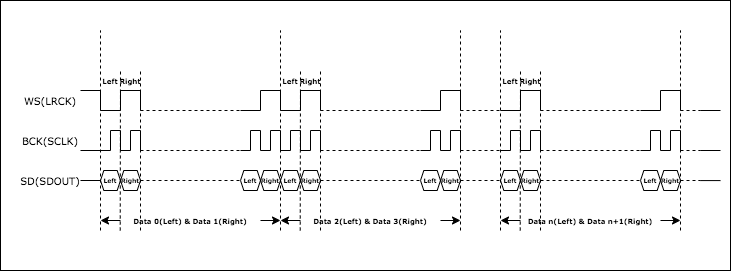
\includegraphics[width=1.0\textwidth]{03-I2S/figures/i2s_pdm_mode.png}
    \caption{PDM Standard Timing Diagram}
    \label{Figure:i2s_pdm_mode}
\end{figure}

\section{TX/RX Clock}\label{The Clock of I2S Module}

I2S\regindex{n}\_TX/RX\_CLK as shown in Figure \ref{Figure:i2s_clk} is the master clock of I2S\regindex{n} TX/RX unit, divided from:
\begin{itemize}
    \item 40 MHz XTAL\_CLK
    \item 160 MHz PLL\_F160M\_CLK
    \item 240 MHz PLL\_D2\_CLK
    \item or external input clock: I2S\regindex{n}\_MCLK\_in
\end{itemize}
%The serial clock (BCK) of the I2S\regindex{n} TX/RX unit is divided from I2S\regindex{n}\_TX/RX\_CLK, as shown in Figure \ref{Figure:i2s_clk}.

\hyperref[fielddesc:I2SRXCLKSEL]{I2S\_TX/RX\_CLK\_SEL} is used to select clock source for TX/RX unit, and \hyperref[fielddesc:I2SRXCLKACTIVE]{I2S\_TX/RX\_CLK\_ACTIVE} to enable or disable the clock source.

\begin{figure}[H]
    \centering
    \fbox{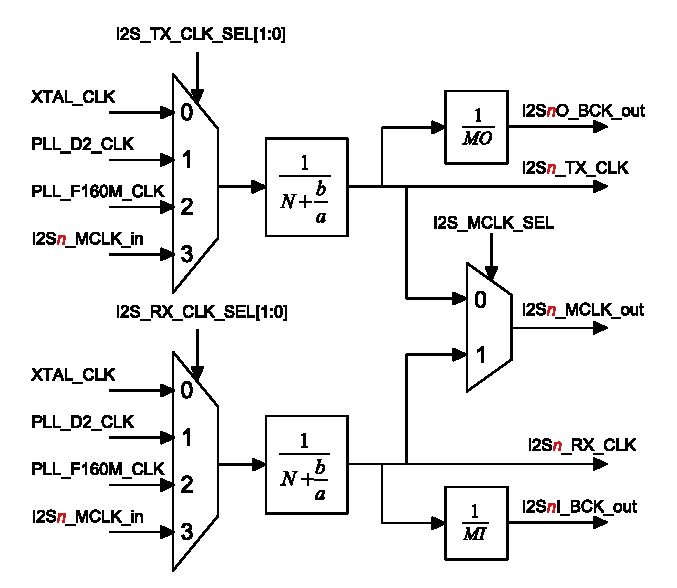
\includegraphics[width=0.6\textwidth]{03-I2S/figures/i2s_clk_20220729}}
    \caption{I2S\regindex{n} Clock}
    \label{Figure:i2s_clk}
\end{figure}


The following formula shows the relation between I2S\regindex{n}\_TX/RX\_CLK frequency ($f_{\textrm{I2S\regindex{n}\_TX/RX\_CLK}}$) and the divider clock source frequency ($f_{\textrm{I2S\regindex{n}\_CLK\_S}}$):
$$f_{\textrm{I2S\regindex{n}\_TX/RX\_CLK}}=\frac{f_{\textrm{I2S\regindex{n}\_CLK\_S}}}{\textrm{N} + \frac{\textrm{b}}{\textrm{a}}}$$

N is an integer value between 2 and 256. The value of N corresponds to the value of  \hyperref[fielddesc:I2STXCLKMDIVNUM]{I2S\_TX/RX\_CLKM\_DIV\_NUM} in register  \hyperref[regdesc:I2STXCLKMCONFREG]{I2S\_TX/RX\_CLKM\_CONF\_REG} as follows:

\begin{itemize}
    \item When  \hyperref[fielddesc:I2STXCLKMDIVNUM]{I2S\_TX/RX\_CLKM\_DIV\_NUM} = 0, N = 256.
    \item When  \hyperref[fielddesc:I2STXCLKMDIVNUM]{I2S\_TX/RX\_CLKM\_DIV\_NUM} = 1, N = 2.
    \item When  \hyperref[fielddesc:I2STXCLKMDIVNUM]{I2S\_TX/RX\_CLKM\_DIV\_NUM} has any other value, N =  \hyperref[fielddesc:I2STXCLKMDIVNUM]{I2S\_TX/RX\_CLKM\_DIV\_NUM}.

\end{itemize}

The values of ``a" and ``b" in fractional divider depend only on x, y, z, and yn1. The corresponding formulas are as follows:
\begin{itemize}
    \item When $\textrm{b} <= \frac{\textrm{a}}{2}$ , $\textrm{yn1} = 0$, $\textrm{x} = floor([\frac{\textrm{a}}{\textrm{b}}]) - 1$, $\textrm{y} = \textrm{a}\%\textrm{b}$, $\textrm{z} = \textrm{b}$;
    \item When $\textrm{b} > \frac{\textrm{a}}{2}$ , $\textrm{yn1}=1$, $\textrm{x} = floor([\frac{\textrm{a}}{\textrm{a - b}}]) - 1$, $\textrm{y} = \textrm{a}\%\textrm{(a - b)}$, $\textrm{z}=\textrm{a - b}$.
\end{itemize}

The values of x, y, z, and yn1 are configured in  \hyperref[fielddesc:I2STXCLKMDIVX]{I2S\_TX/RX\_CLKM\_DIV\_X}, \hyperref[fielddesc:I2STXCLKMDIVY]{I2S\_TX/RX\_CLKM\_DIV\_Y}, \hyperref[fielddesc:I2STXCLKMDIVZ]{I2S\_TX/RX\_CLK\\M\_DIV\_Z}, and \hyperref[fielddesc:I2STXCLKMDIVYN1]{I2S\_TX/RXCLKM\_DIV\_YN1}.

To configure the integer divider, clear \hyperref[fielddesc:I2STXCLKMDIVX]{I2S\_TX/RX\_CLKM\_DIV\_X} and  \hyperref[fielddesc:I2STXCLKMDIVZ]{I2S\_TX/RX\_CLKM\_DIV\_Z}, then set \hyperref[fielddesc:I2STXCLKMDIVY]{I2S\_TX/RX\_C\\LKM\_DIV\_Y} to 1.

\begin{tiplisting}
Using fractional divider may introduce some clock jitter.
\end{tiplisting}

The serial clock (BCK) of the I2S\regindex{n} TX/RX unit is divided from I2S\regindex{n}\_TX/RX\_CLK, as shown in Figure \ref{Figure:i2s_clk}.

In master TX mode, the serial clock BCK for I2S\regindex{n} TX unit is I2S\regindex{n}O\_BCK\_out, divided from I2S\regindex{n}\_TX\_CLK. That is:

$$f_{\textrm{I2S\regindex{n}O\_BCK\_out}} = \frac{f_{\textrm{I2S\regindex{n}\_TX\_CLK}}}{\textrm{MO}}$$


``MO" is an integer value:
$$ \textrm{MO} = \textrm{\hyperref[fielddesc:I2STXBCKDIVNUM]{I2S\_TX\_BCK\_DIV\_NUM}} + 1 $$

{\bfseries Note: }

\hyperref[fielddesc:I2STXBCKDIVNUM]{I2S\_TX\_BCK\_DIV\_NUM} must not be configured as 1.

In master RX mode, the serial clock BCK for I2S\regindex{n} RX unit is I2S\regindex{n}I\_BCK\_out, divided from I2S\regindex{n}\_RX\_CLK. That is:

$$f_{\textrm{I2S\regindex{n}I\_BCK\_out}} = \frac{f_{\textrm{I2S\regindex{n}\_RX\_CLK}}}{\textrm{MI}}$$

``MI" is an integer value:
$$ \textrm{MI} = \textrm{\hyperref[fielddesc:I2STXBCKDIVNUM]{I2S\_RX\_BCK\_DIV\_NUM}} + 1 $$


{\bfseries Note: }
\begin{itemize}
    \item \hyperref[fielddesc:I2SRXBCKDIVNUM]{I2S\_RX\_BCK\_DIV\_NUM} must not be configured as 1.
    \item In slave mode, make sure $f_{\textrm{I2S\regindex{n}\_TX/RX\_CLK}}$ >= 8 * $f_{\textrm{BCK}}$. I2S\regindex{n} module can output I2S\regindex{n}\_MCLK\_out as the master clock for peripherals.

\end{itemize}

\section{I2S\regindex{n} Reset} \label{i2s_module_reset}

The units and FIFOs in I2S\regindex{n} module are reset by the following bits.
\begin{itemize}
\item I2S\regindex{n} TX/RX units: reset by the bits  \hyperref[fielddesc:I2STXRESET]{I2S\_TX\_RESET} and  \hyperref[fielddesc:I2SRXRESET]{I2S\_RX\_RESET}.
\item I2S\regindex{n} TX/RX FIFO: reset by the bits  \hyperref[fielddesc:I2STXFIFORESET]{I2S\_TX\_FIFO\_RESET} and  \hyperref[fielddesc:I2SRXFIFORESET]{I2S\_RX\_FIFO\_RESET}.
\end{itemize}


{\bfseries Note:}
I2S\regindex{n} module clock must be configured first before the module and FIFO are reset.


\section{I2S\regindex{n} Master/Slave Mode}

The \chipname{} I2S\regindex{n} module can operate as a master or a slave, depending on the configuration of \hyperref[fielddesc:I2STXSLAVEMOD]{I2S\_TX\_SLAVE\_MOD} and \hyperref[fielddesc:I2SRXSLAVEMOD]{I2S\_RX\_SLAVE\_MOD}.


\begin{itemize}
    \item \hyperref[fielddesc:I2STXSLAVEMOD]{I2S\_TX\_SLAVE\_MOD}
    \begin{itemize}
        \item 0: master TX mode
        \item 1: slave TX mode
    \end{itemize}
    \item \hyperref[fielddesc:I2SRXSLAVEMOD]{I2S\_RX\_SLAVE\_MOD}
    \begin{itemize}
        \item 0: master RX mode
        \item 1: slave RX mode
    \end{itemize}
\end{itemize}

\subsection{Master/Slave TX Mode} \label{subsubsection:master/slave_transmitting_mode}
\begin{itemize}
    \item I2S\regindex{n} works as a master transmitter:
    \begin{itemize}
        \item Set the bit  \hyperref[fielddesc:I2STXSTART]{I2S\_TX\_START} to start transmitting data.
        \item TX unit keeps driving the clock signal and serial data.
        \item If  \hyperref[fielddesc:I2STXSTOPEN]{I2S\_TX\_STOP\_EN} is set and all the data in FIFO is transmitted, the master stops transmitting data.
        \item If  \hyperref[fielddesc:I2STXSTOPEN]{I2S\_TX\_STOP\_EN} is cleared and all the data in FIFO is transmitted, meanwhile no new data is filled into FIFO, then the TX unit keeps sending the last data frame.
        \item Master stops sending data when the bit  \hyperref[fielddesc:I2STXSTART]{I2S\_TX\_START} is cleared.
    \end{itemize}
    \item I2S\regindex{n} works as a slave transmitter:
     \begin{itemize}
        \item Set the bit  \hyperref[fielddesc:I2STXSTART]{I2S\_TX\_START}.
        \item Wait for the master BCK clock to enable a transmit operation.
        \item If  \hyperref[fielddesc:I2STXSTOPEN]{I2S\_TX\_STOP\_EN} is set and all the data in FIFO is transmitted, then the slave keeps sending zeros, till the master stops providing BCK signal.
        \item If  \hyperref[fielddesc:I2STXSTOPEN]{I2S\_TX\_STOP\_EN} is cleared and all the data in FIFO is transmitted, meanwhile no new data is filled into FIFO, then the TX unit keeps sending the last data frame.
        \item If  \hyperref[fielddesc:I2STXSTART]{I2S\_TX\_START} is cleared, slave keeps sending zeros till the master stops providing BCK clock signal.
    \end{itemize}
\end{itemize}

\subsection{Master/Slave RX Mode}
\begin{itemize}
    \item I2S\regindex{n} works as a master receiver:
    \begin{itemize}
        \item Set the bit  \hyperref[fielddesc:I2SRXSTART]{I2S\_RX\_START} to start receiving data.
        \item RX unit keeps outputting clock signal and sampling input data.
        \item RX unit stops receiving data when the bit  \hyperref[fielddesc:I2SRXSTART]{I2S\_RX\_START} is cleared.
    \end{itemize}
    \item I2S\regindex{n} works as a slave receiver:
     \begin{itemize}
        \item Set the bit  \hyperref[fielddesc:I2SRXSTART]{I2S\_RX\_START}.
        \item Wait for master BCK signal to start receiving data.
        \item RX unit stops receiving data when the bit  \hyperref[fielddesc:I2SRXSTART]{I2S\_RX\_START} is cleared.
    \end{itemize}
\end{itemize}

\section{Transmitting Data}\label{TXCHAN}

\begin{tiplisting}
Updating the configuration described in this and subsequent sections requires to set  \hyperref[fielddesc:I2STXUPDATE]{I2S\_TX\_UPDATE} accordingly, to synchronize I2S\regindex{n} TX registers from APB clock domain to TX clock domain. For more detailed configuration, see Section  \ref{sec:configure-i2s-as-tx-mode}.
\end{tiplisting}
\vspace{-2em}
In TX mode, I2S\regindex{n} first reads data from DMA and sends these data out via output signals according to the configured data mode and channel mode.
\subsection{Data Format Control}
Data format is controlled in the following phases:
\begin{itemize}
    \item Phase I: read data from memory and write it to TX FIFO.
    \item Phase II: read the data to send (TX data) from TX FIFO and convert the data according to output data mode.
    \item Phase III: clock out the TX data serially.
\end{itemize}

\subsubsection{Bit Width Control of Channel Valid Data}
The bit width of valid data in each channel is determined by \hyperref[fielddesc:I2STXBITSMOD]{I2S\_TX\_BITS\_MOD} and  \hyperref[fielddesc:I2STX24FILLEN]{I2S\_TX\_24\_FILL\_EN}, see the table below.

\begin{table}[H]
    \centering
    \caption{Bit Width of Channel Valid Data}
    \label{table:TX_BITS_MODE}
    \begin{threeparttable}
    \begin{tabular}{|p{4.2cm}|R{3.1cm}|R{3.5cm}|}
    \hline
    \rowcolor{lightgray}
    \textbf{Channel Valid Data Width} & \textbf{\hyperref[fielddesc:I2STXBITSMOD]{I2S\_TX\_BITS\_MOD}}  & \textbf{\hyperref[fielddesc:I2STX24FILLEN]{I2S\_TX\_24\_FILL\_EN}} \\ \hline
    \multirow{2}*{32} & 31 & x\tnote{1} \\\cline{2-3}
                      & 23 & 1 \\\hline

                24    & 23 & 0 \\\hline

                16     & 15 & x \\\hline
                8     & 7 & x \\\hline
    \end{tabular}
            \begin{tablenotes}
            \item [1] x: This value is ignored.
        \end{tablenotes}

    \end{threeparttable}
\end{table}

\subsubsection{Endian Control of Channel Valid Data}
When I2S\regindex{n} reads data from DMA, the data endian under various data width is controlled by \hyperref[fielddesc:I2STXBIGENDIAN]{I2S\_TX\_BIG\_ENDIAN}, see the table below.

\begin{table}[H]
    \centering
    \caption{Endian of Channel Valid Data}
    \label{tab:byte-order-control-of-valid-data}
    \begin{tabular}{|p{3.2cm}|p{2.7cm}|p{3.2cm}|R{3.5cm}|}
    \hline
    \rowcolor{lightgray}
    \textbf{Channel Valid Data Width} & \textbf{Origin Data}  & \textbf{Endian of Processed Data}  & \textbf{\hyperref[fielddesc:I2STXBIGENDIAN]{I2S\_TX\_BIG\_ENDIAN}} \\ \hline
    \multirow{2}*{32} & \multirow{2}*{\{B3, B2, B1, B0\}} & \{B3, B2, B1, B0\} & 0 \\\cline{3-4}
                      && \{B0, B1, B2, B3\} & 1 \\\hline

    \multirow{2}*{24} & \multirow{2}*{\{B2, B1, B0\}} & \{B2, B1, B0\} & 0 \\\cline{3-4}
                      && \{B0, B1, B2\} & 1 \\\hline

    \multirow{2}*{16} & \multirow{2}*{\{B1, B0\}} & \{B1, B0\} & 0 \\\cline{3-4}
                      && \{B0, B1\} & 1 \\\hline

                8     & \{B0\} & \{B0\} & x \\\hline
    \end{tabular}
\end{table}

\subsubsection{A-law/$\mu$-law Compression and Decompression}

\chipname{} I2S\regindex{n} compresses/decompresses the valid data into 32-bit by A-law or by $\mu$-law. If the bit width of valid data is smaller than 32, zeros are filled to the extra high bits of the data to be compressed/decompressed by default.

\begin{tiplisting}
Extra high bits here mean the bits[31: channel valid data width] of the data to be compressed/decompressed.
\end{tiplisting}

Configure  \hyperref[fielddesc:I2STXPCMBYPASS]{I2S\_TX\_PCM\_BYPASS} to:
\begin{itemize}
\item 0, do not compress or decompress the data.
\item 1, compress or decompress the data.
\end{itemize}
Configure  \hyperref[fielddesc:I2STXPCMCONF]{I2S\_TX\_PCM\_CONF} to:
\begin{itemize}
\item 0, decompress the data using A-law.
\item 1, compress the data using A-law.
\item 2, decompress the data using $\mu$-law.
\item 3, compress the data using $\mu$-law.
\end{itemize}
At this point, the first phase of data format control is complete.

\subsubsection{Bit Width Control of Channel TX Data}
The TX data width in each channel is determined by \hyperref[fielddesc:I2STXTDMCHANBITS]{I2S\_TX\_TDM\_CHAN\_BITS}.

\begin{itemize}
\item If TX data width in each channel is larger than the valid data width, zeros will be filled to these extra bits. Configure  \hyperref[fielddesc:I2STXLEFTALIGN]{I2S\_TX\_LEFT\_ALIGN} to:
\begin{itemize}
\item 0, the valid data is at the lower bits of TX data.
\item 1, the valid data is at the higher bits of TX data.
\end{itemize}
\item If the TX data width in each channel is smaller than the valid data width, only the lower bits of valid data are sent out, and the higher bits are discarded.
\end{itemize}
At this point, the second phase of data format control is complete.

\subsubsection{Bit Order Control of Channel Data}
The data bit order in each channel is controlled by  \hyperref[fielddesc:I2STXBITORDER]{I2S\_TX\_BIT\_ORDER}:
\begin{itemize}
\item 1, data is sent out from low bits to high bits.
\item 0, data is sent out from high bits to low bits.
\end{itemize}
At this point, the data format control is complete. Figure  \ref{Figure:i2s_data_mode_control} shows a complete process of TX data format control.


\begin{figure}[H]
    \centering
    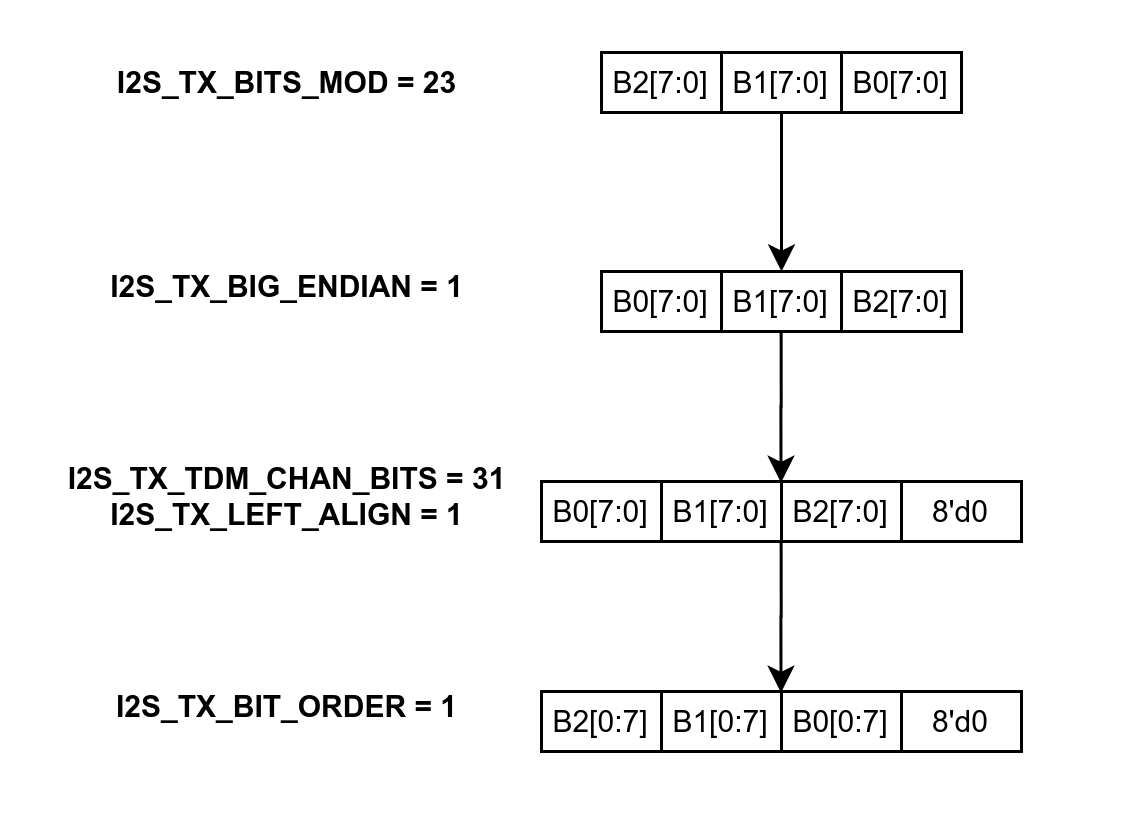
\includegraphics[width=0.8\textwidth]{03-I2S/figures/i2s_tx_data_config.png}
    \caption{TX Data Format Control}
    \label{Figure:i2s_data_mode_control}
\end{figure}

\subsection{Channel Mode Control}
\chipname{} I2S\regindex{n} supports both TDM TX mode and PDM TX mode. Set  \hyperref[fielddesc:I2STXTDMEN]{I2S\_TX\_TDM\_EN} to enable TDM TX mode, or set  \hyperref[fielddesc:I2STXPDMEN]{I2S\_TX\_PDM\_EN} to enable PDM TX mode.

\begin{tiplisting}
\vspace{-2em}
\begin{itemize}
    \item \hyperref[fielddesc:I2STXTDMEN]{I2S\_TX\_TDM\_EN} and \hyperref[fielddesc:I2STXPDMEN]{I2S\_TX\_PDM\_EN} must not be cleared or set simultaneously.
    \item Most stereo I2S codecs can be controlled by setting the I2S\regindex{n} module into 2-channel mode under TDM standard.
    \end{itemize}
\end{tiplisting}

\subsubsection{I2S\regindex{n} Channel Control in TDM Mode} \label{sec:tdm-channel-mode}
In TDM mode, I2S\regindex{n} supports up to 16 channels to output data. The total number of TX channels in use is controlled by  \hyperref[fielddesc:I2STXTDMTOTCHANNUM]{I2S\_TX\_TDM\_TOT\_CHAN\_NUM}. For example, if  \hyperref[fielddesc:I2STXTDMTOTCHANNUM]{I2S\_TX\_TDM\_TOT\_CHAN\_NUM} is set to 5, six channels in total (channel 0 \verb+~+ 5) will be used to transmit data, see Figure
\ref{Figure:i2s_tdm_channel_control}.

In these TX channels, if  \hyperref[fielddesc:I2STXTDMCHAN0EN]{I2S\_TX\_TDM\_CHAN{\textcolor{red}{n}}\_EN} is set to:
\begin{itemize}
    \item 1, this channel sends the channel data out.
    \item 0, the TX data to be sent by this channel is controlled by  \hyperref[fielddesc:I2STXCHANEQUAL]{I2S\_TX\_CHAN\_EQUAL}:
    \begin{itemize}
        \item 1, the data of previous channel is sent out.
        \item 0, the data stored in  \hyperref[fielddesc:I2SSINGLEDATA]{I2S\_SINGLE\_DATA} is sent out.
    \end{itemize}
\end{itemize}
In TDM master mode, WS signal is controlled by \hyperref[fielddesc:I2STXWSIDLEPOL]{I2S\_TX\_WS\_IDLE\_POL} and  \hyperref[fielddesc:I2STXTDMWSWIDTH]{I2S\_TX\_TDM\_WS\_WIDTH}: \begin{itemize}
\item \hyperref[fielddesc:I2STXWSIDLEPOL]{I2S\_TX\_WS\_IDLE\_POL}: the default level of WS signal
\item \hyperref[fielddesc:I2STXTDMWSWIDTH]{I2S\_TX\_TDM\_WS\_WIDTH}: the cycles the WS default level lasts for when transmitting all channel data  \end{itemize}

\hyperref[fielddesc:I2STXHALFSAMPLEBITS]{I2S\_TX\_HALF\_SAMPLE\_BITS} x 2 is equal to the BCK cycles in one WS period.

\textbf{TDM Channel Configuration Example}

In this example, the register configuration is as follows.

\begin{itemize}
    \item \hyperref[fielddesc:I2STXTDMTOTCHANNUM]{I2S\_TX\_TDM\_TOT\_CHAN\_NUM} = 5, i.e. channel 0 \verb+~+ 5 are used to transmit data.
    \item \hyperref[fielddesc:I2STXCHANEQUAL]{I2S\_TX\_CHAN\_EQUAL} = 1, i.e. that data of previous channel will be transmitted if the bit \hyperref[fielddesc:I2STXTDMCHAN0EN]{I2S\_TX\_TDM\_CHAN{\textcolor{red}{n}}\_EN} is cleared. \regindex{n} = 0 \verb+~+ 5.
    \item \hyperref[fielddesc:I2STXTDMCHAN0EN]{I2S\_TX\_TDM\_CHAN0/2/5\_EN} = 1, i.e. these channels send their channel data out.
    \item \hyperref[fielddesc:I2STXTDMCHAN0EN]{I2S\_TX\_TDM\_CHAN1/3/4\_EN} = 0, i.e. these channels send the previous channel data out.
\end{itemize}

Once the configuration is done, data is transmitted as follows.

\begin{figure}[H]
    \centering
    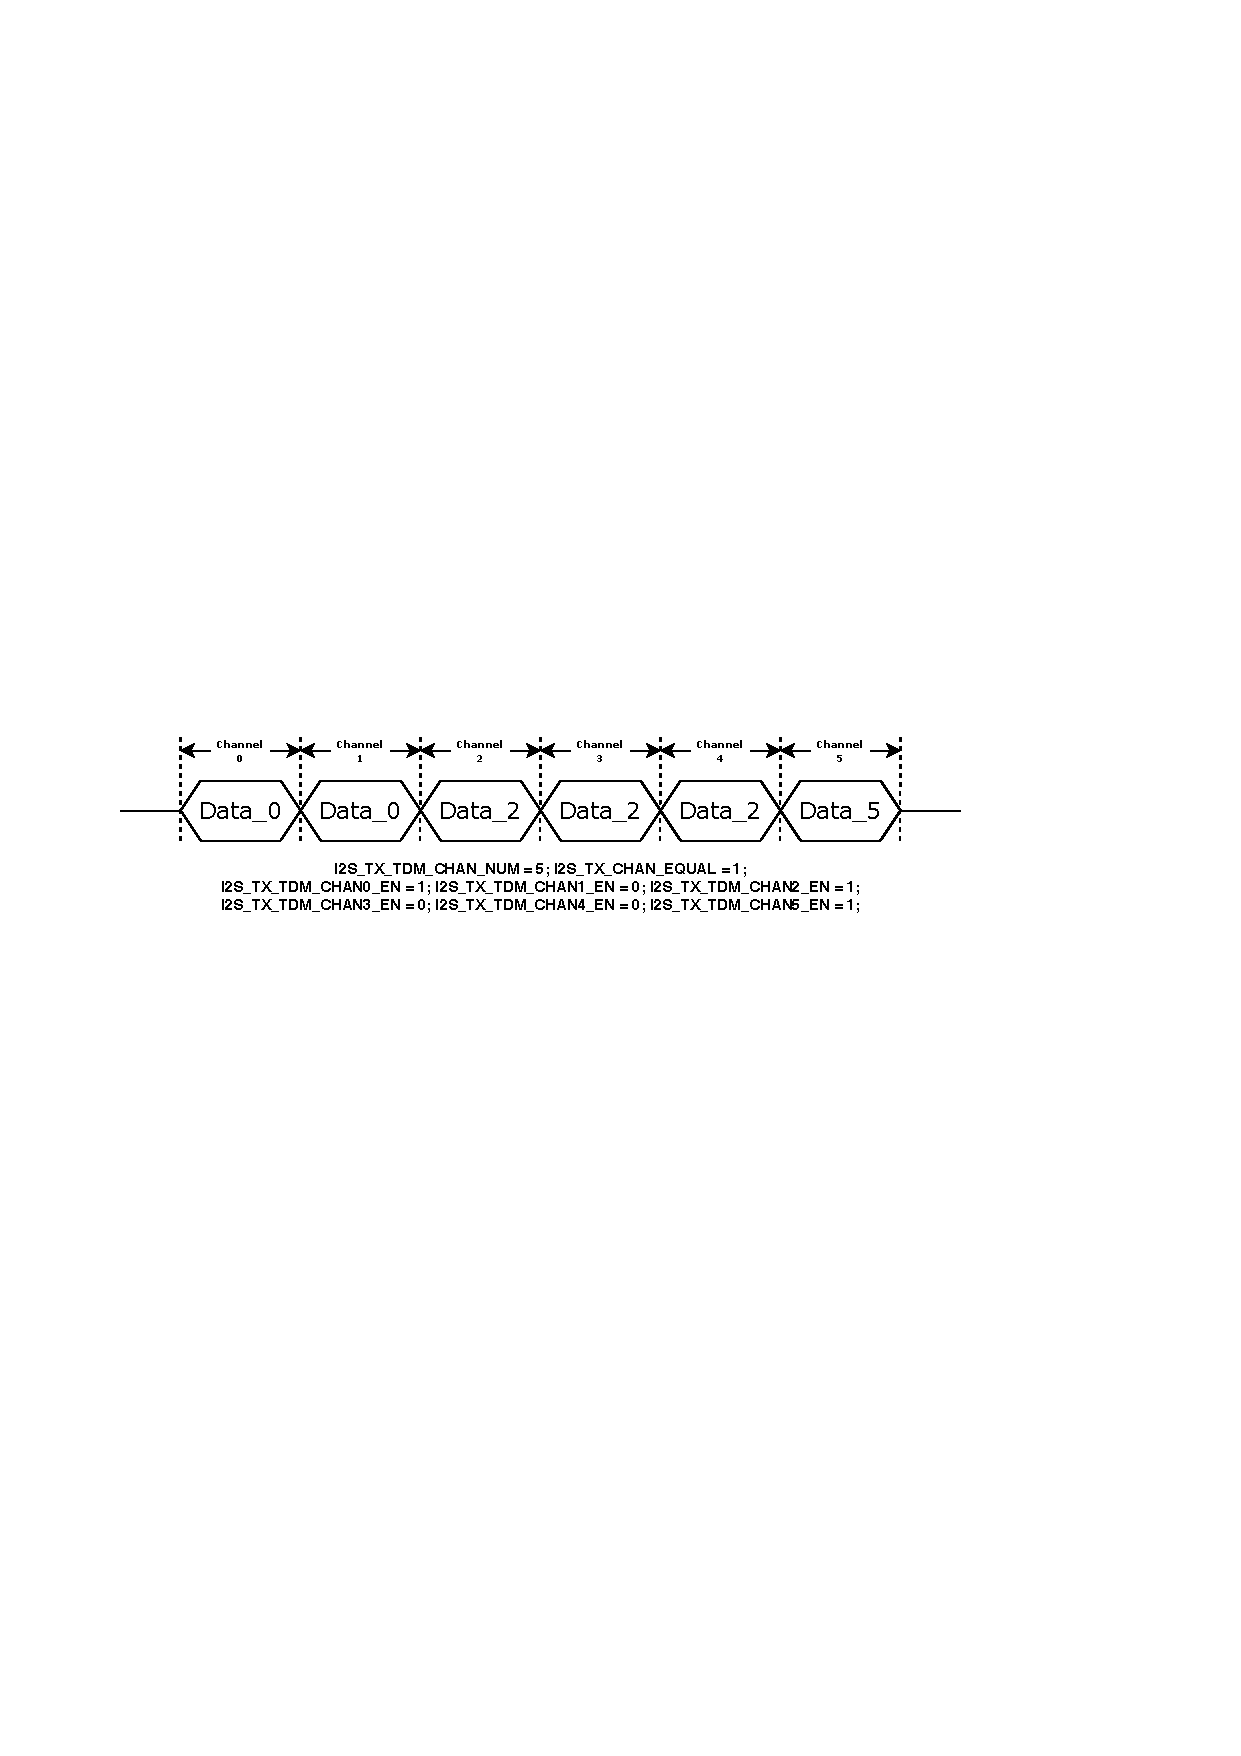
\includegraphics[width=1.0\textwidth]{03-I2S/figures/i2s_tdm_channel_config.pdf}
    \caption{TDM Channel Control}
    \label{Figure:i2s_tdm_channel_control}
\end{figure}


\subsubsection{I2S\regindex{n} Channel Control in PDM Mode}
In PDM mode, fetching data from DMA is controlled by \hyperref[fielddesc:I2STXMONO]{I2S\_TX\_MONO} and  \hyperref[fielddesc:I2STXMONOFSTVLD]{I2S\_TX\_MONO\_FST\_VLD}, see the table below. Please configure the two bits according to the data stored in memory, be it the single-channel or dual-channel data.

\begin{table}[H]
    \centering
    \caption{Data-Fetching Control in PDM Mode}
    \label{table:TX_PDM_DATA_READ}
    \begin{tabular}{|p{6.6cm}|l|r|r|}
    \hline
    \rowcolor{lightgray}
    \textbf{Data-Fetching Control Option} &\textbf{Mode} &\textbf{\hyperref[fielddesc:I2STXMONO]{I2S\_TX\_MONO}}  & \textbf{\hyperref[fielddesc:I2STXMONOFSTVLD]{I2S\_TX\_MONO\_FST\_VLD}} \\ \hline
                        Post data-fetching request to DMA at any edge of WS signal &Stereo mode  & 0  & x \\ \hline
                        Post data-fetching request to DMA only at the second half period of WS signal  & Mono mode  & 1 & 0   \\ \hline
                        Post data-fetching request to DMA only at the first half period of WS signal  & Mono mode  & 1 & 1   \\ \hline
    \end{tabular}
\end{table}
In PDM mode, I2S\regindex{n} channel mode is controlled by  \hyperref[fielddesc:I2STXCHANMOD]{I2S\_TX\_CHAN\_MOD} and \hyperref[fielddesc:I2STXWSIDLEPOL]{I2S\_TX\_WS\_IDLE\_POL}, see the table below.

\begin{table}[H]
    \centering
    \caption{I2S\regindex{n} Channel Control in PDM Mode}
    \label{table:TX_PDM_DATA}
    \begin{threeparttable}
    \begin{tabular}{|p{2.0cm}|L{3.8cm}|L{3.8cm}|R{2.2cm}|R{2.0cm}|}
    \hline
    \rowcolor{lightgray}
    \textbf{Channel Control Option} & \textbf{Left Channel} &\textbf{Right Channel} & \textbf{Mode Control Field}\tnote{1} & \textbf{Channel Select Bit}\tnote{2}\\ \hline
    Stereo mode  & Transmit the left channel data & Transmit the right channel data &0 & x \\\hline
                         \multirow{8}*{Mono mode}  & Transmit the left channel data & Transmit the left channel data & 1 & 0         \\ \cline{2-5}
                                           & Transmit the right channel data & Transmit the right channel data & 1 & 1\\ \cline{2-5}
                                           & Transmit the right channel data & Transmit the right channel data & 2 & 0 \\ \cline{2-5}
                                           & Transmit the left channel data & Transmit the left channel data &2 & 1 \\ \cline{2-5}
                                           & Transmit the value of \hyperref[fielddesc:I2SSINGLEDATA]{I2S\_SINGLE\_DATA} & Transmit the right channel data & 3 & 0 \\ \cline{2-5}
                                           & Transmit the left channel data & Transmit the value of \hyperref[fielddesc:I2SSINGLEDATA]{I2S\_SINGLE\_DATA} &3 & 1 \\ \cline{2-5}
                                           & Transmit the left channel data & Transmit the value of \hyperref[fielddesc:I2SSINGLEDATA]{I2S\_SINGLE\_DATA} &4 & 0 \\ \cline{2-5}
                                           & Transmit the value of \hyperref[fielddesc:I2SSINGLEDATA]{I2S\_SINGLE\_DATA} & Transmit the right channel data & 4 & 1 \\ \hline
    \end{tabular}
            \begin{tablenotes}
            \item[1] \hyperref[fielddesc:I2STXCHANMOD]{I2S\_TX\_CHAN\_MOD}
            \item[2] \hyperref[fielddesc:I2STXWSIDLEPOL]{I2S\_TX\_WS\_IDLE\_POL}
            %\item [3] The ``single” value is equal to the value of  \hyperref[fielddesc:I2SSINGLEDATA]{I2S\_SINGLE\_DATA}.
        \end{tablenotes}

    \end{threeparttable}
\end{table}


In PDM master mode, the WS level of I2S\regindex{n} module is controlled by  \hyperref[fielddesc:I2STXWSIDLEPOL]{I2S\_TX\_WS\_IDLE\_POL}. The frequency of WS signal is half of BCK frequency. The configuration of WS signal is similar to that of BCK signal, see Section  \ref{The Clock of I2S Module} and Figure  \ref{Figure:i2s_channel_mode}.

\chipname{} I2S\regindex{0} also supports PCM-to-PDM output mode, in which the PCM data from DMA is converted to PDM data and then output in PDM signal format. Configure  \hyperref[fielddesc:I2SPCM2PDMCONVEN]{I2S\_PCM2PDM\_CONV\_EN} to enable this mode.

The register configuration for PCM-to-PDM output mode is as follows:

\begin{itemize}
    \item Configure 1-line PDM output format or 1-/2-line DAC output mode as the table below:

\begin{table}[H]
    \centering
    \caption{PCM-to-PDM Output Mode}
    \label{table:PDM_TX_MODE}
    \begin{threeparttable}
    \begin{tabular}{|p{4.3cm}|R{5.2cm}|R{5.0cm}|}
    \hline
    \rowcolor{lightgray}
    \textbf{Channel Output Format}&\textbf{\hyperref[fielddesc:I2STXPDMDACMODEEN]{I2S\regindex{0}\_TX\_PDM\_DAC\_MODE\_EN}} & \textbf{\hyperref[fielddesc:I2STXPDMDAC2OUTEN]{I2S\regindex{0}\_TX\_PDM\_DAC\_2OUT\_EN}}\\ \hline
    1-line PDM output format\tnote{1}& 0 & x \\ \hline
    1-line DAC output format\tnote{2} &1   & 0  \\ \hline
    2-line DAC output format & 1 & 1 \\ \hline
    \end{tabular}
    \begin{tablenotes}
    \item[1] In PDM output format, SD data of two channels is sent out in one WS period.
    \item[2] In DAC output format, SD data of one channel is sent out in one WS period.
    \end{tablenotes}
        \end{threeparttable}
\end{table}
    \item Configure sampling frequency and upsampling rate \newline
    In PCM-to-PDM mode, PDM clock frequency is equal to BCK frequency. The relation of sampling frequency ($f_{\textrm{Sampling}}$) and BCK frequency is as follows:
    $$f_{\textrm{Sampling}} = \frac{f_{\textrm{BCK}}}{\textrm{OSR}}$$

    Upsampling rate (OSR) is related to \hyperref[fielddesc:I2STXPDMSINCOSR2]{I2S\regindex{0}\_TX\_PDM\_SINC\_OSR2} as follows:
    $${\textrm{OSR}} = {\textrm{\hyperref[fielddesc:I2STXPDMSINCOSR2]{I2S\regindex{0}\_TX\_PDM\_SINC\_OSR2}}} \times {\textrm{64}}$$

    Sampling frequency $f_{\textrm{Sampling}}$ is related to \hyperref[fielddesc:I2STXPDMFS]{I2S\_TX\_PDM\_FS} as follows:
    $$f_{\textrm{Sampling}} = {\textrm{\hyperref[fielddesc:I2STXPDMFS]{I2S\regindex{0}\_TX\_PDM\_FS}}} \times {\textrm{100}}$$

    Configure the registers according to needed sampling frequency, upsampling rate, and PDM clock frequency.
\end{itemize}

\textbf{PDM Channel Configuration Example}

In this example, the register configuration is as follows.
\begin{itemize}
    \item \hyperref[fielddesc:I2STXCHANMOD]{ I2S\_TX\_CHAN\_MOD} = 2, i.e. mono mode is selected.
    \item  \hyperref[fielddesc:I2STXWSIDLEPOL]{I2S\_TX\_WS\_IDLE\_POL} = 1, i.e. both the left channel and right channel transmit the left channel data.
\end{itemize}

Once the configuration is done, the channel data is transmitted as follows.

\begin{figure}[H]
    \centering
    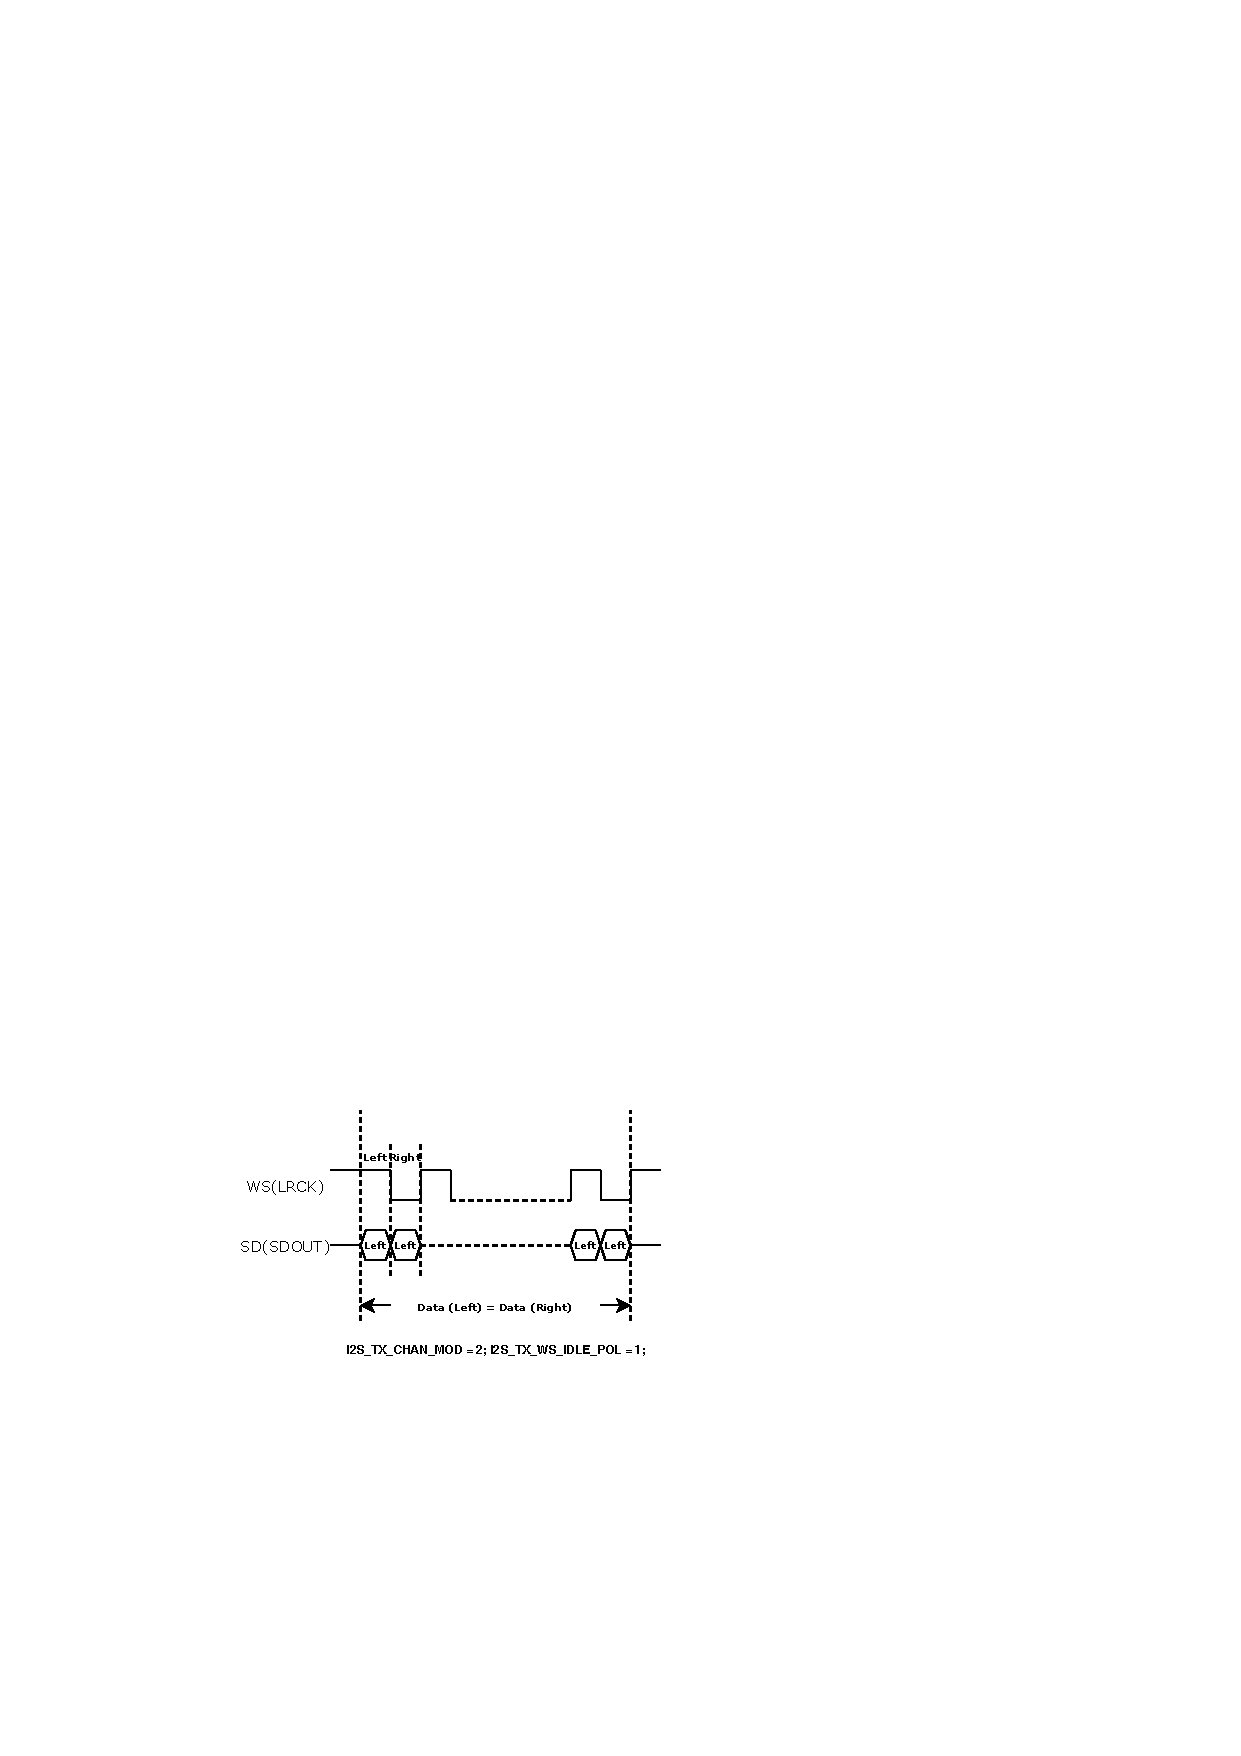
\includegraphics[width=0.8\textwidth]{03-I2S/figures/i2s_chan_mode_20220210.pdf}
    \caption{PDM Channel Control}
    \label{Figure:i2s_channel_mode}
\end{figure}

\section{Receiving Data}\label{RXCHAN}
\begin{tiplisting}
Updating the configuration described in this and subsequent sections requires to set  \hyperref[fielddesc:I2SRXUPDATE]{I2S\_RX\_UPDATE} accordingly, to synchronize I2S\regindex{n} RX registers from APB clock domain to RX clock domain. For more detailed configuration, see Section  \ref{sec:configure-i2s-as-rx-mode}.
\end{tiplisting}
\vspace{-2em}
In RX mode, I2S\regindex{n} first reads data from peripheral interface, and then stores the data into memory via DMA, according to the configured channel mode and data mode.

\subsection{Channel Mode Control}
\chipname{} I2S\regindex{n} supports both TDM RX mode and PDM RX mode. Set  \hyperref[fielddesc:I2SRXTDMEN]{I2S\_RX\_TDM\_EN} to enable TDM RX mode, or set  \hyperref[fielddesc:I2SRXPDMEN]{I2S\_RX\_PDM\_EN} to enable PDM RX mode.

\textbf{Note}: \hyperref[fielddesc:I2SRXTDMEN]{I2S\_RX\_TDM\_EN} and  \hyperref[fielddesc:I2SRXPDMEN]{I2S\_RX\_PDM\_EN} must not be cleared or set simultaneously.

\subsubsection{I2S\regindex{n} Channel Control in TDM Mode}
In TDM mode, I2S\regindex{n} supports up to 16 channels to input data. The total number of RX channels in use is controlled by  \hyperref[fielddesc:I2SRXTDMTOTCHANNUM]{I2S\_RX\_TDM\_TOT\_CHAN\_NUM}. For example, if  \hyperref[fielddesc:I2SRXTDMTOTCHANNUM]{I2S\_RX\_TDM\_TOT\_CHAN\_NUM} is set to 5, channel 0 \verb+~+ 5 will be used to receive data.

In these RX channels, if  \hyperref[fielddesc:I2STXTDMCHAN0EN]{I2S\_RX\_TDM\_CHAN{\textcolor{red}{n}}\_EN}  is set to:
\begin{itemize}
    \item 1, this channel data is valid and will be stored into RX FIFO.
    \item 0, this channel data is invalid and will not be stored into RX FIFO.
\end{itemize}
In TDM master mode, WS signal is controlled by  \hyperref[fielddesc:I2SRXWSIDLEPOL]{I2S\_RX\_WS\_IDLE\_POL} and  \hyperref[fielddesc:I2SRXTDMWSWIDTH]{I2S\_RX\_TDM\_WS\_WIDTH}:
\begin{itemize}
\item \hyperref[fielddesc:I2SRXWSIDLEPOL]{I2S\_RX\_WS\_IDLE\_POL}: the default level of WS signal
\item \hyperref[fielddesc:I2SRXTDMWSWIDTH]{I2S\_RX\_TDM\_WS\_WIDTH}: the cycles the WS default level lasts for when receiving all channel data
\end{itemize} \hyperref[fielddesc:I2SRXHALFSAMPLEBITS]{I2S\_RX\_HALF\_SAMPLE\_BITS} x 2 is equal to the BCK cycles in one WS period.


\subsubsection{I2S\regindex{n} Channel Control in PDM Mode}
In PDM mode, I2S\regindex{n} converts the serial data from channels to the data to be entered into memory.

In PDM master mode, the WS level of I2S\regindex{n} module is controlled by  \hyperref[fielddesc:I2SRXWSIDLEPOL]{I2S\_RX\_WS\_IDLE\_POL}. WS frequency is half of BCK frequency. The configuration of BCK signal is similar to that of WS signal as described in Section  \ref{The Clock of I2S Module}. Note, in PDM RX mode, the value of  \hyperref[fielddesc:I2SRXHALFSAMPLEBITS]{I2S\_RX\_HALF\_SAMPLE\_BITS} must be same as that of  \hyperref[fielddesc:I2SRXBITSMOD]{I2S\_RX\_BITS\_MOD}.

I2S\regindex{0} supports PDM-to-PCM input mode, in which the received PDM data is converted to PCM data and controlled according to the data mode. Configure  \hyperref[fielddesc:I2SRXPDM2PCMEN]{I2S\_RX\_PDM2PCM\_EN} to enable this mode.


The register configuration for PDM-to-PCM input mode is as follows:

\begin{itemize}
    \item Configure sampling frequency and downsampling rate.\newline
    In PDM-to-PCM input mode, PDM clock frequency is:
    \begin{itemize}
        \item in master mode: PDM clock frequency is equal to BCK frequency.
        \item in slave mode: PDM clock is provided by external device.
    \end{itemize}
    The sampling frequency ($f_{\textrm{Sampling}}$) is related to PDM clock frequency as follows:
    $$f_{\textrm{Sampling}} = \frac{f_{\textrm{PDM}}}{\textrm{DSR}}$$
    Downsampling rate (DSR) is related to \hyperref[fielddesc:I2SRXPDMSINCDSR16EN]{I2S\regindex{0}\_RX\_PDM\_SINC\_DSR\_16\_EN} as follows:
    $${\textrm{DSR}} = {\textrm{\hyperref[fielddesc:I2SRXPDMSINCDSR16EN]{I2S\regindex{0}\_RX\_PDM\_SINC\_DSR\_16\_EN}}} \times {\textrm{64}}$$
    Configure the registers according to needed master/slave mode, sampling frequency, and downsampling rate.
    \item Configure valid channels. \newline
    In PDM-to-PCM mode, input signals from eight channels are supported at most. See Table \ref{table:PDM_RX_MODE} for the register configuration and related channels.
\begin{table}[H]
    \centering
    \caption{PDM-to-PCM Input Mode}
    \label{table:PDM_RX_MODE}
    \begin{tabular}{|p{4.0cm}|p{2.3cm}|p{5.8cm}|}
    \hline
    \rowcolor{lightgray}
    \textbf{Input Data Signal}&\textbf{Channel} &\textbf{Enable Register} \\ \hline
    \multirow{2}*{I2S\regindex{0}I\_Data\_in}  & Left channel & \hyperref[fielddesc:I2SRXTDMPDMCHAN0EN]{I2S\regindex{0}\_RX\_TDM\_PDM\_CHAN0\_EN} \\ \cline{2-3}
                                               & Right channel & \hyperref[fielddesc:I2SRXTDMPDMCHAN0EN]{I2S\regindex{0}\_RX\_TDM\_PDM\_CHAN1\_EN} \\ \hline
    \multirow{2}*{I2S\regindex{0}I1\_Data\_in} & Left channel & \hyperref[fielddesc:I2SRXTDMPDMCHAN0EN]{I2S\regindex{0}\_RX\_TDM\_PDM\_CHAN2\_EN} \\ \cline{2-3}
                                               & Right channel & \hyperref[fielddesc:I2SRXTDMPDMCHAN0EN]{I2S\regindex{0}\_RX\_TDM\_PDM\_CHAN3\_EN} \\ \hline
    \multirow{2}*{I2S\regindex{0}I2\_Data\_in} & Left channel & \hyperref[fielddesc:I2SRXTDMPDMCHAN0EN]{I2S\regindex{0}\_RX\_TDM\_PDM\_CHAN4\_EN} \\ \cline{2-3}
                                               & Right channel & \hyperref[fielddesc:I2SRXTDMPDMCHAN0EN]{I2S\regindex{0}\_RX\_TDM\_PDM\_CHAN5\_EN} \\ \hline
    \multirow{2}*{I2S\regindex{0}I3\_Data\_in} & Left channel & \hyperref[fielddesc:I2SRXTDMPDMCHAN0EN]{I2S\regindex{0}\_RX\_TDM\_PDM\_CHAN6\_EN} \\ \cline{2-3}
                                               & Right channel & \hyperref[fielddesc:I2SRXTDMPDMCHAN0EN]{I2S\regindex{0}\_RX\_TDM\_PDM\_CHAN7\_EN} \\ \hline
    \end{tabular}
\end{table}
\end{itemize}


\subsection{Data Format Control}
Data format is controlled in the following phases:
\begin{itemize}
    \item Phase I: serial input data is converted into the data to be saved to RX FIFO.
    \item Phase II: the data is read from RX FIFO and converted according to input data mode.
\end{itemize}

\subsubsection{Bit Order Control of Channel Data}
The data bit order in each channel is controlled by  \hyperref[fielddesc:I2SRXBITORDER]{I2S\_RX\_BIT\_ORDER}:
\begin{itemize}
\item 1, serial data is entered from low bits to high bits.
\item 0, serial data is entered from high bits to low bits.
\end{itemize}
At this point, the first phase of data format control is complete.

\subsubsection{Bit Width Control of Channel Storage (Valid) Data}
The storage data width in each channel is controlled by \hyperref[fielddesc:I2SRXBITSMOD]{I2S\_RX\_BITS\_MOD} and  \hyperref[fielddesc:I2SRX24FILLEN]{I2S\_RX\_24\_FILL\_EN}, see the table below.

\begin{table}[H]
    \centering
    \caption{Channel Storage Data Width}
    \label{table:RX_BITS_MODE}
    \begin{tabular}{|p{3cm}|R{3.3cm}|R{4cm}|}
    \hline
    \rowcolor{lightgray}
    \textbf{Channel Storage Data Width} & \textbf{\hyperref[fielddesc:I2SRXBITSMOD]{I2S\_RX\_BITS\_MOD}} & \textbf{\hyperref[fielddesc:I2SRX24FILLEN]{I2S\_RX\_24\_FILL\_EN}}  \\ \hline
    \multirow{2}*{32} & 31 & x \\\cline{2-3}
                 & 23 & 1 \\ \hline
    24 & 23 & 0 \\\hline
    16    & 15 & x \\\hline
    8     & 7 & x \\\hline
    \end{tabular}
\end{table}

\subsubsection{Bit Width Control of Channel RX Data}
The RX data width in each channel is determined by \hyperref[fielddesc:I2SRXTDMCHANBITS]{I2S\_RX\_TDM\_CHAN\_BITS}.
\begin{itemize}
\item If the storage data width in each channel is smaller than the received (RX) data width, then only the bits within the storage data width is saved into memory. Configure  \hyperref[fielddesc:I2STXLEFTALIGN]{I2S\_RX\_LEFT\_ALIGN} to:
\begin{itemize}
\item 0, only the lower bits of the received data within the storage data width is stored to memory.
\item 1, only the higher bits of the received data within the storage data width is stored to memory.
\end{itemize}
\item If the received data width is smaller than the storage data width in each channel, the higher bits of the received data will be filled with zeros and then the data is saved to memory.
\end{itemize}

\subsubsection{Endian Control of Channel Storage Data}
The received data is then converted into storage data (to be stored to memory) after some processing, such as dis- carding extra bits or filling zeros in missing bits. The endian of the storage data is controlled by \hyperref[fielddesc:I2SRXBIGENDIAN]{I2S\_RX\_BIG\_ENDIAN} under various data width, see the table below.
\begin{table}[H]
    \centering
    \caption{Channel Storage Data Endian}
    \label{table:TX_BIG_ENDIAN}
    \begin{tabular}{|p{3cm}|p{3cm}|p{3.5cm}|R{3.5cm}|}
    \hline
    \rowcolor{lightgray}
        \textbf{Channel Storage Data Width} & \textbf{Origin Data} & \textbf{Endian of Processed Data} & \textbf{\hyperref[fielddesc:I2SRXBIGENDIAN]{I2S\_RX\_BIG\_ENDIAN}} \\ \hline
 \multirow{2}*{32} & \multirow{2}*{\{B3, B2, B1, B0\}} & \{B3, B2, B1, B0\} & 0 \\\cline{3-4}
                      && \{B0, B1, B2, B3\} & 1 \\\hline

    \multirow{2}*{24} & \multirow{2}*{\{B2, B1, B0\}} & \{B2, B1, B0\} & 0 \\\cline{3-4}
                      && \{B0, B1, B2\} & 1 \\\hline

    \multirow{2}*{16} & \multirow{2}*{\{B1, B0\}} & \{B1, B0\} & 0 \\\cline{3-4}
                      && \{B0, B1\} & 1 \\\hline

                8     & \{B0\} & \{B0\} & x \\\hline
    \end{tabular}
\end{table}

\subsubsection{A-law/$\mu$-law Compression and Decompression}

\chipname{} I2S\regindex{n} compresses/decompresses the data to be stored in 32-bit by A-law or by $\mu$-law. By default, zeros are filled to high bits.

Configure  \hyperref[fielddesc:I2SRXPCMBYPASS]{I2S\_RX\_PCM\_BYPASS} to:
\begin{itemize}
\item 0, do not compress or decompress the data.
\item 1, compress or decompress the data.
\end{itemize}
Configure  \hyperref[fielddesc:I2SRXPCMCONF]{I2S\_RX\_PCM\_CONF} to:
\begin{itemize}
\item 0, decompress the data using A-law.
\item 1, compress the data using A-law.
\item 2, decompress the data using $\mu$-law.
\item 3, compress the data using $\mu$-law.
\end{itemize}
At this point, the data format control is complete. Data then is stored into memory via DMA.

\section{Software Configuration Process}
\subsection{Configure I2S\regindex{n} as TX Mode}\label{sec:configure-i2s-as-tx-mode}
Follow the steps below to configure I2S\regindex{n} as TX mode via software:

\begin{enumerate}
    \item Configure the clock as described in Section  \ref{The Clock of I2S Module}.

    \item Configure signal pins according to Table  \ref{table:I2S 信号总线描述}.

    \item Select the mode needed by configuring the bit  \hyperref[fielddesc:I2STXSLAVEMOD]{I2S\_TX\_SLAVE\_MOD}.
    \begin{itemize}
        \item 0: master TX mode
        \item 1: slave TX mode
    \end{itemize}

    \item Set needed TX data mode and TX channel mode as described in Section  \ref{TXCHAN}, and then set the bit  \hyperref[fielddesc:I2STXUPDATE]{I2S\_TX\_UPDATE}.

    \item Reset TX unit and TX FIFO as described in Section  \ref{i2s_module_reset}.
    \item Enable corresponding interrupts, see Section  \ref{I2S_INT}.\label{I2S-TX-INTERRUPT}
    \item Configure DMA outlink.

    \item Set  \hyperref[fielddesc:I2STXSTOPEN]{I2S\_TX\_STOP\_EN} if needed. For more information, please refer to Section  \ref{subsubsection:master/slave_transmitting_mode}.

    \item Start transmitting data:
    \begin{itemize}
        \item In master mode, wait till I2S\regindex{n} slave gets ready, then set  \hyperref[fielddesc:I2STXSTART]{I2S\_TX\_START} to start transmitting data.
        \item In slave mode, set the bit  \hyperref[fielddesc:I2STXSTART]{I2S\_TX\_START}. When the I2S\regindex{n} master supplies BCK and WS signals, I2S\regindex{n} slave starts transmitting data.
    \end{itemize}

    \item Wait for the interrupt signals set in Step  \ref{I2S-TX-INTERRUPT}, or check whether the transfer is completed by querying  \hyperref[fielddesc:I2STXIDLE]{I2S\_TX\_IDLE}:
    \begin{itemize}
        \item 0: transmitter is working.
        \item 1: transmitter is in idle.
    \end{itemize}

    \item Clear  \hyperref[fielddesc:I2STXSTART]{I2S\_TX\_START} to stop data transfer.
\end{enumerate}
\subsection{ Configure I2S\regindex{n} as RX Mode}\label{sec:configure-i2s-as-rx-mode}
Follow the steps below to configure I2S\regindex{n} as RX mode via software:

\begin{enumerate}
    \item Configure the clock as described in Section  \ref{The Clock of I2S Module}.

    \item Configure signal pins according to Table  \ref{table:I2S 信号总线描述}.

    \item Select the mode needed by configuring the bit \hyperref[fielddesc:I2SRXSLAVEMOD]{ I2S\_RX\_SLAVE\_MOD}.
    \begin{itemize}
        \item 0: master RX mode
        \item 1: slave RX mode
    \end{itemize}

    \item Set needed RX data mode and RX channel mode as described in Section  \ref{RXCHAN}, and then set the bit  \hyperref[fielddesc:I2SRXUPDATE]{I2S\_RX\_UPDATE}.

    \item Reset RX unit and its FIFO according to Section  \ref{i2s_module_reset}.
    \item Enable corresponding interrupts, see Section  \ref{I2S_INT}.\label{I2S-RX-INTERRUPT}

    \item Configure DMA inlink, and set the length of RX data in  \hyperref[regdesc:I2SRXEOFNUMREG]{I2S\_RXEOF\_NUM\_REG}.

    \item Start receiving data:
    \begin{itemize}
        \item In master mode, when the slave is ready, set  \hyperref[fielddesc:I2SRXSTART]{I2S\_RX\_START} to start receiving data.
        \item In slave mode, set  \hyperref[fielddesc:I2SRXSTART]{I2S\_RX\_START} to start receiving data when get BCK and WS signals from the master.
    \end{itemize}
    \item The received data is then stored to the specified address of  \chipname{} memory according the configuration of DMA. Then the corresponding interrupt set in Step  \ref{I2S-RX-INTERRUPT} is generated.
\end{enumerate}


\section{I2S\regindex{n} Interrupts} \label{I2S_INT}

\begin{itemize}
\item \label{int:I2STXHUNGINT}I2S\_TX\_HUNG\_INT: triggered when transmitting data is timed out. For example, if I2S\regindex{n} module is configured as TX slave mode, but the master does not provide BCK or WS signal for time specified in  \hyperref[regdesc:I2SLCHUNGCONFREG]{I2S\_LC\_HUNG\_CONF\_REG}, then this interrupt will be triggered.
\item \label{int:I2SRXHUNGINT}I2S\_RX\_HUNG\_INT: triggered when receiving data is timed out. For example, if I2S\regindex{n} module is configured as RX slave mode, but the master does not send data for time specified in  \hyperref[regdesc:I2SLCHUNGCONFREG]{I2S\_LC\_HUNG\_CONF\_REG}, then this interrupt will be triggered.
\item \label{int:I2STXDONEINT}I2S\_TX\_DONE\_INT: triggered when transmitting data is completed.
\item \label{int:I2SRXDONEINT}I2S\_RX\_DONE\_INT: triggered when receiving data is completed.
\end{itemize}

\hypertarget{i2s-reg-summ}{}
\section{Register Summary}

The addresses in this section are relative to [I2S\regindex{n}] base address provided in Table \ref{tab:sysmem-base-address} in Chapter \ref{mod:sysmem} \textit{\nameref{mod:sysmem}}.

The abbreviations given in Column \textbf{Access} are explained in Section \hyperref[glossary-access-types]{\textit{Access Types for Registers}}.

\subfile{03-I2S/03-I2S-reg-summ__EN}

\section{Registers}\label{I2SRegister}
\subfile{03-I2S/03-I2S-reg__EN}
\end{document}